% 映射
% 单射|满射|函数|一一对应|定义域|值域|逆映射

\pentry{集合\upref{Set}}

给定集合 $A$ 和 $B$,我们可以从$A$中每一个元素上拉一根线连接到 $B$ 中的某一个元素,这些线的分布形式就被称为一个从 $A$ 到 $B$ 的\textbf{映射(mapping)}, 也叫\textbf{算符(operator)}.将这个映射记为 $f$, $A$ 中拉出线的元素组成的集合,叫做 $f$ 的\textbf{定义域(domain)}, $B$ 中被线连接到的元素的集合,叫做 $f$ 的\textbf{值域}或\textbf{像(image)}. 我们一般将 “$f$ 是从 $A$ 到 $B$ 的映射” 记为
\begin{equation}
f:A\to B
\end{equation}
也就是说从 $A$ 的元素上拉线到 $B$ 的元素上. 如果没有特殊说明,这样的表示方法都默认 $f$ 的定义域是整个 $A$ 集合. 有时候, 为了表示映射的定义域 $A$ 是另一个集合的 $S$ 的子集, 我们也会将映射记为
\begin{equation}
f: A\subseteq S \to B
\end{equation}
注意映射是有方向区分的,比如在上面的例子中, $A$ 中每个元素都有且只有一根线拉出去, 但是 $B$ 中的元素可以同时被一根或多根线连接的, 也可以没有连接(即不在值域中).

如果映射 $f:A \to B$ 中每个 $B$ 中元素只被1根或者0根线连接,那么称$f$是一个\textbf{单射(injective)}. 如果$f:A→ B$中每个$B$中元素都被至少1根线连接, 那么称$f$是一个\textbf{满射(surjection)}. 如果 $f$ 既是单射又是满射,那么称它为一个\textbf{双射(bijective)}, 或者叫\textbf{一一对应(one to one)}.

% \textbf{Cantor-Bernstein 定理}显示,如果集合$A$到集合$B$上存在一个单射$f$和一个满射$g$,那么总可以利用$f$和$g$来构造出一个双射. 未完成: 应该新开词条

\begin{figure}[ht]
\centering
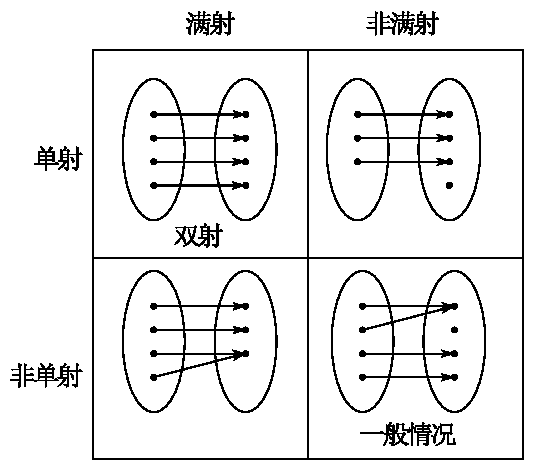
\includegraphics[width=8cm]{./figures/map_1.pdf}
\caption{映射的分类} \label{map_fig1}
\end{figure}

如果 $f:A\to B$ 是一个双射,那么 $A$ 中每一个元素都唯一地连接到 $B$ 中某一个元素,并且 $B$ 中每一个元素也都唯一被 $A$ 中某一个元素所连接,因此很明显可以将这个过程反过来,从 $B$ 中向 $A$ 中拉连接线.另外,如果 $A$ 和 $B$ 存在双射,意味着 $A$ 和 $B$ 的元素数量应该一致\footnote{本书中统一使用这种定义. 一些其他教材中也把我们的 “单射” 称为 “一一映射”, 把 “满射” 称为 “到上”, 把 “双射” 称为 “一一到上”, 需要特别小心.}.

函数是一种常见的映射, 例如 $f(x) = 2x$ 可以看作映射 $f: \mathbb R \to \mathbb R$. 但是映射可以从任意集合到任意集合. 例如将整数映射到正多边形, 将函数的映射到函数或实数(一般把这种映射称为\textbf{算符})等.

注意当一个集合中有无限个元素时, 我们有可能在它的子集和它本身之间建立一一映射, 例如函数 $\tan(x)$ 可以从实轴的开区间 $(-\pi/2, \pi/2)$ 一一映射到整个实轴 $\mathbb R$, 又例如我们可以将全体整数 $\mathbb Z$ 乘以二后一一映射到全体偶数 $2\mathbb Z$ 上. 这时我们仍然认为这两个集合的元素一样多, 虽然直觉上可能不容易接受.

\subsection{相等和拓展}
当映射(算符) $f:A\to B$ 和 $g:C\to D$ 的定义域相等($A = C$)且对任意 $x\in A$ 都有 $fx = gx$, 那么我们就说两个映射(算符)\textbf{相等}, 记为 $f = g$, 否则它们就不相等.

若 $A$ 是 $C$ 的子集($A\subseteq C$), 我们就说 $g$ 是 $f$ 的\textbf{拓展(extension)}, 记为 $f \subseteq g$. 特殊地, 当 $A$ 是 $C$ 的真子集($A\subset C$), 就记为 $f \subset g$.

\subsection{复合映射}
给定两个映射 $f:A\to B$ 和 $g:C\to D$, 如果 $f$ 的值域 $R$ 是 $g$ 的定义域 $C$ 的一个子集, 则可以定义\textbf{符合映射} $g\circ f: A\to D$, 即先将 $A$ 中的元素通过 $f$ 映射到 $R \subseteq C$, 再通过 $g$ 映射到 $D$ 的元素. 在没有歧义的情况下也可以将 $\circ$ 省略, 尤其是将映射称为\textbf{算符}时.

复合映射常见的例子是复合函数, 令 $\mathbb R$ 上的函数 $f(x) = \sin x$, $g(x) = x^2$, 则复合函数 $g\circ f: \mathbb R \to [0, 1]$ 为 $(g\circ f)(x) = g(f(x)) = \sin^2 x$.

根据定义, 复合映射满足分配律, 令 $f, g, h$ 为映射, 则
\begin{equation}
h \circ (g \circ f) = (h \circ g) \circ f
\end{equation}

\subsection{恒等映射和逆映射}
若一个集合到它子集的映射 $f:X\to X$ 把任意 $x\in X$ 映射到 $x$ 本身, 我们就叫它\textbf{恒等映射(identity map)}或者\textbf{单位算符(unit operator)}, 通常用 $I$ 或 $E$ 表示. 注意对不同集合 $X$, 它们的单位算符定义域并不相等, 所以它们的单位算符也不相等.

对于任意单射 $f:A\to B$, 令其值域为 $R \subseteq B$, 那么 $f:A\to R$ 就是一一映射, 所以我们总可以唯一地定义其逆映射 $f^{-1}:R \subseteq B \to A$.

所以对于一一映射 $f:A\to B$, 显然 $f\circ f^{-1}$ 和 $f^{-1}\circ f$ 都是单位算符. 注意两者的定义域分别为 $A$ 和 $B$, 当 $A \ne B$ 时不能写成 $f\circ f^{-1} = f^{-1}\circ f$.

\begin{example}{}
如果取正弦函数 $y = \sin x$ 的值域为 $R = [-1, 1]$ 如果取定义域为 $\mathbb R$,  那么它不是一个单射, 因为每一个 $y \in R$ 都对应无穷个 $x$, 所以不存在反函数. 但如果取定义域为 $[-\pi/2, \pi/2]$, 那么它是一个单射, 存在反三角函数 $\sin^{-1}: [-1, 1] \to [-\pi/2, \pi]$.

根据以上定义, $\sin^{-1} (\sin(x))$ 是定义在 $[-\pi/2, \pi/2]$ 上的恒等函数, 而 $\sin (\sin^{-1}(x))$ 是定义在 $[-1, 1]$ 上的恒等函数, 所以有 $\sin \circ \sin^{-1} \subseteq \sin^{-1} \circ \sin$.
\end{example}

\subsection{广义逆映射}

给定集合$A, B$,定义$B^A$为“从$A$到$B$的所有可能的映射所构成的集合”.如果$B$是一个二元集合,即它只有两个元素,不妨记为$B=\{0,1\}$,那么$B^A$可以用来表示$A$的\textbf{幂集},即由$A$的所有子集所构成的集合.这是因为对于任意的$f\in B^A$,我们可以把这个$f$对应到$A$的子集$S$,其中$S$的元素全都被$f$映射到1上,$A-S$的元素全都被$f$映射到0上.当然,0和1的地位反过来也可以.由于这个特点,我们简单地把$A$的幂集记为$2^A$. 

对于映射$f:A\to B$,可以定义其逆映射$f^{-1}:B→ 2^A$. 逆映射$f^{-1}$将$B$中的每个元素映射到$A$的某个子集上(而不是$A$的某个元素上).特别地,不在$f$的值域中的元素被$f^{-1}$映射到空集上,而空集也是$A$的一个子集.如果$f$是一个双射,那么$f^{-1}$都映射在$A$的单元素子集上,那么我们也可以认为此时$f^{-1}$实际上是映射在单个元素上,也是从$B$到$A$的映射.
